	\chapter{Dise\~no}\label{cap.desarrollo}
	
	En este capítulo se va a explicar de forma más detallada las características y el funcionamiento de todos los elementos de los que se hará uso para llevar a cabo el desarrollo de este proyecto. Además se detallará el desarrollo hardware, firmware y software, explicando con detalle la configuración electrónica y se presentará la solución software implementada.
	
	A continuación se detalla el diagrama de bloques que representa el proyecto desarrollado:
	
	\begin{figure}[h]
		\centering
		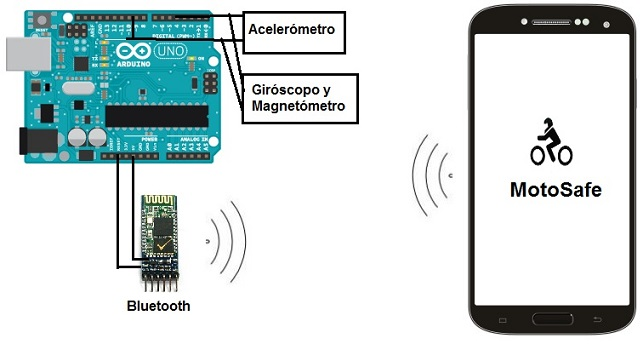
\includegraphics{imagenes/DiagramaBloques.jpg}
		\caption{Diagrama Bloques}
		\label{contexto:figura}
	\end{figure}
	
	Tal y como se puede observar en la figura se observa un módulo Arduino conectado a una unidad inercial que se compone de un acelerómetro y magnetómetros mas un giróscopo. Además posee un módulo bluetooth conectado a la placa Arduino que será el encargado de establecer la comunicación bluetooth con el smartphone para que ésta pueda interpretar los datos medidos por la unidad inercial.
	
	
	\section{Hardware}
	
		En esta sección Los diferentes protocolos de comunicación que podemos usar y los módulos que nos ofrecen dicho servicio. A partir de ahí seleccionaremos cual nos resulta mas interesante para el desarrollo de este proyecto.
		
		
		\subsection{Protocolos de comunicación y módulos}
		
		
			\subsubsection{Protocolo Wi-Fi}
				
				Es la tecnología usada en una red o conexión inalámbrica para la comunicación de datos entre equipos situados dentro de una misma área, interior o exterior, de cobertura. Tiene un alcance de 20 metros en interiores. Usa los estándares IEEE 802.11b, IEEE 802.11g e IEEE 802.11n para la banda de 2,4 GHz, con una velocidad de hasta 300 Mbit/s.
				
				Sus ventajas son:
				
				\begin{itemize}	
					\item Movilidad desde cualquier sitio dentro de su cobertura.
					\item Fácil instalación.
					\item Flexibilidad, permite el acceso a una red en entornos de difícil cableado.
					\item Permite incorporar redes sin la necesidad de cables.
				\end{itemize}
				
				Los módulos que se podrían usar serían los detallados a continuación.
				
				El módulo WiFi ESP8266 \cite{ESP8266} es un auto SOC contenido en la pila de protocolos TCP/IP que puede dar cualquier acceso microcontrolador a tu red WiFi. Cada módulo ESP8266 viene pre-programado con un comando AT, solo se debe conectar a un dispositivo Arduino y obtener casi tanto capacidad WiFi como WiFi Shield. El módulo ESP8266 es extremadamente eficaz.
				
				\begin{figure}[h]
					\centering
					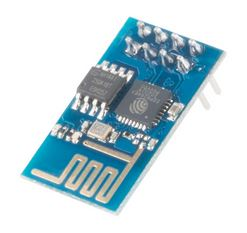
\includegraphics{imagenes/ESP8266.JPG}
					\caption{Módulo WiFi ESP8266}
					\label{contexto:figura}
				\end{figure}
		
				Este módulo tiene una gran alcance ademas de su capacidad de almacenamiento que le permite integrarse con los sensores y dispositivos específicos de la aplicación a través de sus GPIOs con un desarrollo mínimo por adelantado. Su alto grado de integración en el chip permite una circuitería externa mínima, incluyendo el módulo de front-end, está diseñado para ocupar un área mínima de PCB. 
				
				\begin{itemize}	
					
					\item 802.11 b/g/n.
					
					\item Wi-Fi Direct (P2P).
					
					\item Protocolo TCP/IP.
					
				\end{itemize}
		
				El módulo RN-XV \cite{RNXV} DE Roving Networks es una solución certificada Wi-Fi diseñadA especialmente para los clientes que quieran migrar su arquitectura 802.15.4 existente a una plataforma basada en TCP / IP estándar sin tener que rediseñar su hardware existente. En otras palabras, permite configurar su sistema y moverlo a una red Wi-Fi estándar, no se precisa de un hardware nuevo, ya que se puede usar el mismo socket diseñado.
				
				\begin{figure}[h]
					\centering
					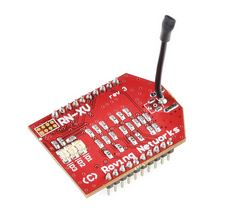
\includegraphics{imagenes/RNXV.JPG}
					\caption{Módulo WiFi RN-XV}
					\label{contexto:figura}
				\end{figure}
				
				Está precargado con Roving firmware para simplificar la integración y reducir al mínimo el tiempo de desarrollo de su aplicación. La configuración es simple, el hardware sólo requiere cuatro conexiones (PWR, TX, RX y GND) para crear una conexión de datos inalámbrica. El módulo RN-XV  se basa en el módulo robusto RN-171 Wi-Fi Roving Networks e incorpora: . 
				
				\begin{itemize}	
					
					\item 802.11 b/g de radio.
					
					\item Pila TCP / IP de 32 bits.
					
					\item Reloj en tiempo real.
					
					\item Unidad de administración de energía.
					
				\end{itemize}
				
				
				
			\subsubsection{Protocolo Zigbee}
			
				ZigBee es un protocolo de comunicaciones inalámbricas basado en el estándar 802.15.4, está pensado para comunicaciones a baja velocidad entre dos o varios dispositivos, se pueden formar redes con miles de dispositivos comunicandose entre sí, por lo que es ideal para muchas aplicaciones.
				
				ZigBee es desarrollado por la ZigBee Alliance, formada por cientos de compañias que quieren solventar la necesidad de un estándar para comunicaciones a baja velocidad, con un bajo coste de implementación y donde los dispositivos que forman parte de una red pueden requerir un bajo consumo, llegando a estar funcionando durante años con un par de pilas.
				
				Las características de las redes/dispositivos ZigBee serían las siguientes:
				
				\begin{itemize}
				\item Velocidad de transmisión entre 25-250 kbps.
				\item Protocolo asíncrono, half duplex y estandarizado, permitiendo a productos de distintos fabricantes trabajar juntos.
				\item Se pueden formar redes que contengan desde dos dispositivos hasta cientos de ellos.
				\item Los dispositivos de estas redes pueden funcionar en un modo de bajo consumo, lo que supone años de duración de sus baterías.
				\item Opera en la frecuencia de 2.4 GHz (16 canales) y también en las frecuencias de 868 MHz y 915 MHz.
				\item Es un protocolo fiable, la red se organiza y se repara de forma automática y se rutean los paquetes de manera dinámica.
				\item Es un protocolo seguro ya que se puede implementar encriptación y autentificación.
				\end{itemize}
				
				Se puede decir que ZigBee ocupa el vacío que hay por debajo de Bluetooth, para comunicaciones de datos que no requieren altas velocidades.
				
				Algunos módulos Zigbee que se podrían usar serían los siguientes.
				
				XBee ZB \cite{xbeeZD} ofrecen conectividad inalámbrica rentable de dispositivos en las redes de malla ZigBee. Utilizando el PRO Feature Set ZigBee, estos módulos son interoperables con otros dispositivos ZigBee, incluyendo los dispositivos de otros fabricantes. Versiones programables del XBee-PRO ZB hacen aplicaciones ZigBee con una personalización fácil, incluso sin experiencia en diseño inalámbrico.
				
				\begin{figure}[h]
					\centering
					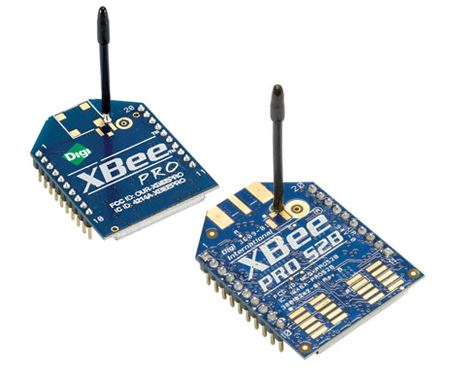
\includegraphics{imagenes/XBEEZD.JPG}
					\caption{Módulo XBee-PRO ZB}
					\label{contexto:figura}
				\end{figure}
				
				Algunas características que posee este módulo son las siguientes:
				
				\begin{itemize}
					\item 250 Kbps.
					\item Entre 40 y 90 metros de alcance.
					\item 2 mW de potencia.
					\item -96 dBm de sensibilidad en recepción.
					\item 2,4 GHz.
				\end{itemize}
				
				El módulo CC2530 F256 Wireless ZigBee \cite{zigbee} reune varios métodos de comunicación en 16 canales. Utilizado habitualmente en una red inalámbrica de sensores, para controlar la casa, el consumo energético o en el sector de la industria.
				
				\begin{figure}[h]
					\centering
					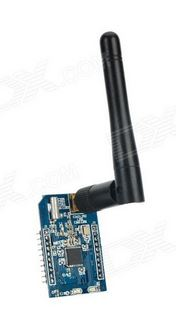
\includegraphics{imagenes/zigbee.JPG}
					\caption{Módulo CC2530 F256 Wireless ZigBee}
					\label{contexto:figura}
				\end{figure}
				
				Posee las siguientes características:
				
				\begin{itemize}
					\item Oscilador de 32,768 KHz y un cristal SMD de 32 MHz.
					\item fuente de alimentación de 3,6 V.
					\item 2,4 GHz.
					\item 70 metros de alcance.
				\end{itemize}
				
			
				
				
			\subsubsection{Protocolo Bluetooth}
			
				Bluetooth es una especificación industrial para Redes Inalámbricas de Área Personal (WPAN) que posibilita la transmisión de voz y datos entre diferentes dispositivos mediante un enlace por radiofrecuencia en la banda ISM de los 2,4 GHz. Los principales objetivos que se pretenden conseguir con esta norma son:
				
				\begin{itemize}
					\item Facilitar las comunicaciones entre equipos móviles.
					\item Eliminar los cables y conectores entre éstos.
					\item Ofrecer la posibilidad de crear pequeñas redes inalámbricas y facilitar la sincronización de datos entre equipos personales.
				\end{itemize}
				
				Para ello vamos a ver los siguientes módulos.
				
				Módulo Bluetooth RN-42 \cite{RN42} está dise\~nado para reemplazar los cables de serie. Está completamente encapsulado, el usuario solo ve los caracteres de serie se transmiten hacia atrás y adelante. Este dispositivo es usado para corto alcance, con un consumo de 26 uA en reposo. Fácil de integrar en sistemas embebidos y de conectar a dispotivos ya existentes 
				
				\begin{figure}[h]
					\centering
					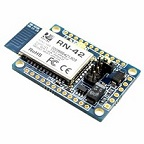
\includegraphics{imagenes/RN42.jpg}
					\caption{Módulo Bluetooth RN-42}
					\label{contexto:figura}
				\end{figure}
				
				\begin{itemize}
					\item Soporte para: BCSP, LAN, GAP, SDP, RFCOMM y L2CAP
					\item Velocidad UART: hasta 3 Mbps
					\item Alcance: 15-18 m 
				\end{itemize}
				
							
				El módulo Bluetooth HC-05 \cite{HC05} ofrece una mejor relación precio frente a prestaciones, es un módulo maestro esclavo, no solo recibe conexiones sino que también las genera hacia otros dispositivos Bluetooth. Posee la versión V2.0+EDR, trabajando a una frecuencia de 2,4 GHz en la banda ISM, con una modulación GFSK.
				
				\begin{itemize}
					\item Soporta comando AT para ser configurado
					\item Velocidad: hasta 2,1 Mbps y Síncrono 1Mbps/1Mbps
					\item Alcance: 10 m 
				\end{itemize}
				
				\begin{figure}[h]
					\centering
					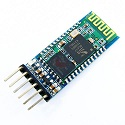
\includegraphics{imagenes/HC05}
					\caption{Módulo Bluetooth HC-05}
					\label{contexto:figura}
				\end{figure}
				
				El alcance teórico es de 10 metros, pero el alcance práctico es de 8,5 metros aproximadamente, medidos en un espacio abierto sin inclemencias meteorológicas.
		
			\subsubsection{Conclusión}
			
			Estudiados estos módulos se decidió usar el módulo Bluetooth HC-05 no solo por ser mas econónico sino porque es un dispositivo que puede seguir trabajando en un rango de temperaturas de -$20^{\circ}$C hasta $75^{\circ}$C y teniendo en cuenta que este sistema estará ubicado en el interior de la moto es posible alcanzar dichas temperaturas. Además las características del módulo HC-05 son sufientes para la realización de este proyecto, atendiendo a la cantidad de información transmitida, alcance máximo y velocidad necesaria.
		
		
		\subsection{Unidad Inercial}
		
			Entre las unidades inerciales encontradas en el mercado, podemos destacar las siguientes.
		
			\subsubsection{Unidad de medición incercial ARDUINO+V2 (FLAT)}
			
				ARDUINO+V2 (FLAT) \cite{FLAT} es una unidad de medición inercial que consiste en un acelerómetro de 3 ejes, tres giroscopios, dos reguladores de voltaje (3,3 V y 5V), un puerto del GPS (compatible con uBlox, EM406 y MediaTek MT3329), un microcontrolador ATMega328 @ 16 MHz y un algunos indicadores LED de estado. El microcontrolador es capaz de ejecutar el codice de Actitud partida del sistema (AHRS), basado en el algoritmo de DCM Bill Premerlani.
				
				\begin{figure}[h]
					\centering
					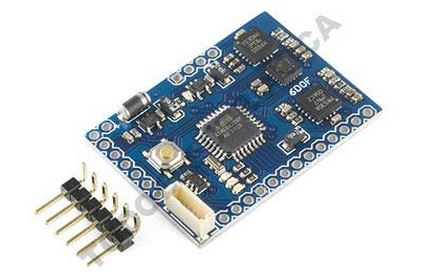
\includegraphics{imagenes/FLAT.JPG}
					\caption{Unidad de medición inercial ARDUINO+V2 (FLAT)}
					\label{contexto:figura}
				\end{figure}
				
				Las características técnicas de dicha unidad son las siguientes:
				
				\begin{itemize}
					\item Acelerómetro de 3 ejes.
					\item Giroscopio de 3 ejes.
					\item Compatibilidad con Arduino.
					\item El código fuente incluido y de código abierto.
					\item LED de encendido (verde).
					\item LEDs de estado (rojo, azul, amarillo).
					\item Un puerto SPI.
					\item 1 puerto I2C.
					\item 2 salidas PWM (los funcionarios).
					\item Puerto GPS.
					\item Protección del diodo.
					\item Conector de puerto serie para el servo estándar (tierra, 5V, TX-OUT).
					\item Peso: 6 gramos.
				\end{itemize}
			
			\subsubsection{Mota Sensora}
				
				Nuesta unidad de medición inercial (IMU), que viene equipada con un L3GD20 giroscopio de 3 ejes y un LSM303DLHC con 3 ejes para el acelerómetro y 3 ejes para el magnetómetro \cite{Pololu}. El módulo incluye un regulador de voltaje y un circuito de desplazamiento que permite el funcionamiento de 2,5 a 5,5 V.
				
				Las especificaciones de la mota son las siguientes:
				
				\begin{itemize}
					\item Dimensiones: 20 x 13 x 3 mm
					\item Peso: 0,7 g
					\item Alimentación: 10 mA 
					\item Giróscocopo: lectura de 16 bits por eje
					\item Acelerómetro: lectura de 12 bits por eje
					\item Magnetómetro: lectura de 12 bits por eje
					\item Rango de sensibilidad configurable
				\end{itemize}
				
				\begin{figure}[h]
					\centering
					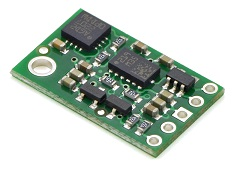
\includegraphics{imagenes/pololu.jpg}
					\caption{Mota sensora}
					\label{contexto:figura}
				\end{figure}
				
				El L3GD20 es un sensor de tres ejes para medir velocidad angular a baja potencia.
				
				Incluye un elemento de detección y una interfaz IC capaz de proporcionar la velocidad angular medida con el exterior a través de una interfaz digital (I2C / SPI).
				
				El sensor está fabricado usando un proceso de micro-mecanizado dedicado al desarrollado por STMicroelectronics para producir sensores inerciales y actuadores de silicio.
				
				La interfaz IC se fabrica utilizando un proceso CMOS que permite un alto nivel de integración para dise\~nar un circuito dedicado que se recorta para adaptarse mejor a las características del elemento de detección. El L3GD20 tiene una escala de 250 - 2.000 dps y es capaz de medir las tasas con un ancho de banda seleccionable por el usuario.
				
				El L3GD20 está disponible en un paquete de plástico y puede operar dentro de un rango de temperatura de -40 a 85 grados centígrados.
				
				El LSM303DLHC es un sistema empaquetado con un sensor lineal digital en 3 ejes de aceleración y un sensor magnético digital en 3 ejes.
				
				El LSM303DLHC tiene escalas lineales llenos de aceleración de 2, 4, 8 y 16 g y un campo magnético a gran escala de 1,3, 1,9, 2,5, 4,0, 4,7, 5,6 y 8,1 gauss.
				
				El LSM303DLHC incluye una interfaz de bus serie I2C que soporta el modo estándar y rápido a 100 kHz y 400 kHz. El sistema puede ser configurado para generar se\~nales de interrupción por eventos, así como por la posición del propio dispositivo. Los umbrales y tiempos de generadores de interrupción son programables por el usuario final. Los bloques magnético y acelerómetro se pueden activar o poner en modo de apagado por separado.
				
				El LSM303DLHC está disponible en un paquete de plástico y puede operar dentro de un rango de temperatura de -40 a 85 grados centígrados.
			
			\subsubsection{Conclusión}
		
				Finalmente se decidió usar nuestra Mota sensora, ya que ofrece una mayor precición, ya que la primera unidad inercial ofrece 6 grados de libretad, 3 pertenecientes al acelerómetro y otros 3 pertenecientes al giroscopio, mientras que nuestra unidad inercial posee 9 grados de libertad, los 6 ya mencionados mas los 3 correspondientes al magnetómetro. Además la diferencia de precio para poder desarrollar estre proyecto era muy elevada, por lo que se decidió usar la Mota sensora.
		
		\subsection{Plataforma de código abierto}
		
		
			\subsubsection{Arduino Uno}
		
				Arduino Uno R3 \cite{ArduinoUno}, placa electrónica basada en el microcontrolador ATmega 328. Cuenta con 14 pines digitales de entrada/salida, 6 entradas analógicas, un resonador cerámico de 16 MHz, una conexión USB, un conector de alimentación, una cabecera ICSP y un botón de reinicio. Basta con conectarlo a un ordenador con un cable USB o a una bateria para empezar.
				
				\begin{figure}[h]
					\centering
					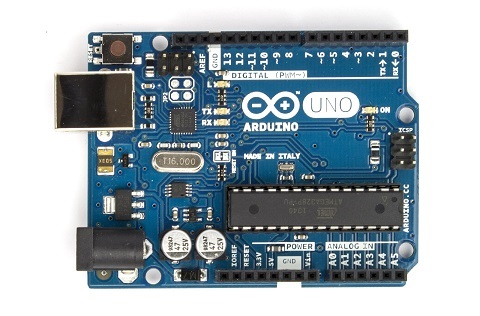
\includegraphics{imagenes/ArduinoUno.jpg}
					\caption{ATmega328 en Arduino Uno R3}
					\label{contexto:figura}
				\end{figure}
				
				Arduino Uno puede ser alimentado con 6 hasta 20 voltios. Si se alimenta con menos de 7 voltios, el pin encargado de suministrar 5 voltios es muy probable que suministre menos. En caso de suministrar mas de 12 voltios, el regulador de voltaje se puede sobrecalentar y da\~nar la placa. El rango de alimentación recomendado es de 7 a 12 voltios.
				
				Para programar Arduino Uno se puede usar el software de Arduino. Software desde el que podremos cargar nuestros programas en la placa Arduino a través de un cable USB, Arduino Uno cuenta con una memoria de 2KB de SRAM y 1 KB de EEPROM.
				
				ATmega328 \cite{ATmega328} es un microcontrolador creado por Atmel y que pertenece a la serie megaAVR. Cabe destacar:   
				
				\begin{itemize}	
					
					\item Es un circuito integrado de alto rendimiento que está basado en un microcontrolador RISC.
					
					\item Combina 32 KB ISP flash de memoria con la capacidad de leer y escribir.
					
					\item 1 KB de memoria EEPROM.
					
					\item 2 KB de SRAM.
					
					\item 23 líneas de E/S de propósito general.
					
					\item 32 registros de proceso general.
					
					\item  Tres temporizadores contadores con modo de comparación.
					
					\item Interrupciones internas y externas.
					
					\item Programador de modo USART.
					
					\item Interfaz serial orientada a byte de 2 cables.
					
					\item SPI puerto serial.
					
					\item 6 canales 10 bit conversor A/D y cinco modos de ahorro de energía seleccionables por software.
					
					\item Opera entre 1,8 y 5,5 voltios.
					
					\item Alcanza una respuesta de 1 MIPS.
					
					\item Consumo balanceando de energía y velocidad de proceso
					
				\end{itemize}
		
			\subsubsection{Raspberry Pi}
			
				Raspberry Pi \cite{RaspBerryPi} es un ordenador de placa reducida o (placa única) (SBC) de bajo coste desarrollado en Reino Unido por la Fundación Raspberry Pi, con el objetivo de estimular la enseñanza de ciencias de la computación en las escuelas.
				
				\begin{figure}[h]
					\centering
					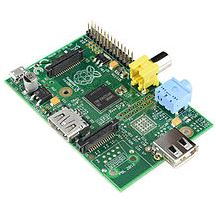
\includegraphics{imagenes/RBPI.JPG}
					\caption{Raspberry Pi Modelo A}
					\label{contexto:figura}
				\end{figure}
				
				El diseño incluye un System-on-a-chip Broadcom BCM2835, que contiene un procesador central (CPU) ARM1176JZF-S a 700 MHz (el firmware incluye unos modos “Turbo” para que el usuario pueda hacerle overclock de hasta 1 GHz sin perder la garantía),9 un procesador gráfico (GPU) VideoCore IV, y 512 MB de memoria RAM (aunque originalmente al ser lanzado eran 256 MB). El diseño no incluye un disco duro ni unidad de estado sólido, ya que usa una tarjeta SD para el almacenamiento permanente; tampoco incluye fuente de alimentación ni carcasa. El 29 de febrero de 2012 la fundación empezó a aceptar órdenes de compra del modelo B, y el 4 de febrero de 2013 del modelo A.
				
				
				
				A pesar que el Modelo A no tiene un puerto RJ45, se puede conectar a una red usando un adaptador USB-Ethernet suministrado por el usuario. Por otro lado, a ambos modelos se puede conectar un adaptador Wi-Fi por USB, para tener acceso a redes inalámbricas o internet. El sistema cuenta con 256 MB de memoria RAM en su modelo A, y con 512 MB de memoria RAM en su modelo B. Como es típico en los ordenadores modernos, se pueden usar teclados y ratones con conexión USB compatible con Raspberry Pi.
			
			\subsubsection{Conclusión}
		
				Arduino y Raspberry Pi, pueden lucir muy parecidas, incluso es posible que hayamos asumido que este par de plataformas de hardware compiten para resolver problemas similares. En realidad son muy diferentes. Para empezar, Raspberry Pi es una computadora completamente funcional, mientras que Arduino es un microcontrolador, el cual es sólo un componente de una computadora.
				
				Las principales diferencias entre Raspberry Pi y Arduino son:
		
				\begin{itemize}	
					
					\item Arduino es básicamente un microcontrolador con el que podemos conectar nuestro ordenador directamente y programar diferentes funciones para sus sensores. En cambio, la placa de Raspberry Pi es un microprocesador o, lo que es lo mismo, un ordenador que dispone de 256 o 512 MB de memoria RAM.
					\item Arduino no tiene un sistema operativo propio.
					\item Arduino no se puede conectar a Internet a menos que se compre una caja con salida de Ethernet.
					\item Raspberry Pi es mas compleja a la hora de hacer proyectos sencillos.
					\item Realizar un proyecto como un Media Center en casa es mucho mas fácil de realizar con una Raspberry Pi que con Arduino.
					\item La velocidad de la placa es superior en Raspberry Pi, ya que cuenta con 700MHz mientras que en Arduino la velocidad es de 16MHz.
					\item Las dos se crearon para proyectos estudiantiles: Arduino para proyectos relacionados con la electrónica y Raspberry Pi para llevar de una forma distinta el conocimiento de la informática.
	
				\end{itemize}
		
				En base a lo expuesto se decidió trabajar con Arduino, ademas na de las ventajas que ofrece Arduino es:
				
				\begin{itemize}
					\item Su bajo coste.
					\item La facilidad para leer los datos suministrados por sensores.
					\item La facilidad para construir el sistema electrónico que deseamos.
				\end{itemize}
		
		
		
			
			
		
		
	\section{Firmware}
	
		En los que respecta al firmware vamos a detallar como hemos configurado cada uno de los dispositivos hardware y conectado entre sí. Mostrando al final un Schematic con todos los componentes conectados y su implementación sobre una protoboax.
		
		\subsection{Configuración Arduino Uno y unidad inercial}
		
			El uso de este sensor en la placa Arduino requería a\~nadir dos librerías en el software que posteriormente cargaríamos en la placa arduino.
			
			Las dos librerías usadas son:
			
			\begin{itemize}	
				
				\item include L3G.h
				
				\item include LSM303.h
				
			\end{itemize}
			
			
			Además hemos usado la librería \#include SoftwareSerial.h, que permite la comunicación entre los pines de la motasensora y de la placa Arduino.
			
			Una vez cargadas dichas librerías inicializamos todas las variables a usar en el código además de los pertinentes métodos para tomar los valores medidos de cada sensor en los 3 ejes. En lo que respecta al código Arduino siempre tendremos dos métodos a usar, como son setup() el encargado de configurar la placa e inicializar los métodos y el método loop(), el cual ejecutará las acciones que le ordenemos de forma reiterativa.
			
			En lo que respecta a las conexiones, conectamos la patilla SDA y SCL con la patilla A4 y A5 respecticamente de la placa Arduino, además de VCC y GND entre la motasensora y la placa.
			
			\begin{figure}[h]
				\centering
				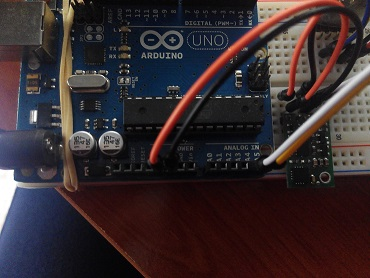
\includegraphics{imagenes/ConfMota.jpg}
				\caption{Conexiones Motasonra y Arduino}
				\label{contexto:figura}
			\end{figure}
			
			
			En lo que respecta a la configuración de la mota sensora, debemos fijarle una posición inicial. Que será con respecto a la cual calculemos los ángulos de inclinación con respecto a la vertical de la moto. Al encender este sistema electrónico se produce un calibrado de los angulos iniciales. 
			
		
		\subsection{Configuración Arduino Uno y Bluetooth HC-05}
	
			El uso del dispositibo bluetooth HC-05 en la placa Arduino requería a\~nadir dos librerías en el software que posteriormente cargaríamos en la placa arduino.
			
			Las librerías usadas son:
			
			\begin{itemize}	
				
				\item include SoftwareSerial.h
				
				\item include wire.h
				
			\end{itemize}
			
			En nuestro código Arduino debemos dejar indicado que el pin RXD es el 10 y el pin TDX es el 11 con el siguiente comando:
			
			SoftwareSerial BT = SoftwareSerial(10, 11); //10 RX, 11 TX.
			
			Además debemos configurar el Arduino para que el pin 10 sea de entrada y el pin 11 de salida, indicando en el PinMode si es InPut o OutPut respectivamente. Ambos componentes se deben comunicar a 9600 baudios, velocidad por defecto de funcionamiento del bluetooth HC-05, una configuración a una velocidad diferente provoca que no haya comunicación entre el dispositivo bluetooth y la placa Arduino.
			
			\begin{figure}[h]
				\centering
				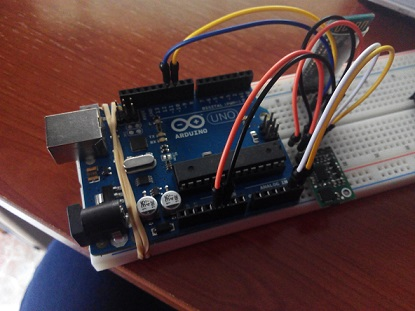
\includegraphics{imagenes/implementacion.jpg}
				\caption{Resultado conexión todos los componentes}
				\label{contexto:figura}
			\end{figure}
			
			En lo que respecta a las conexiones, la patilla RXD y TXD del módulo bluetooth se conectarán a las patillas 11 y 12 respectivamente de la placa Arduino, además de VCC y GND entre el módulo bluetooth y la placa.
			
			En los que respecta al método loop() de nuestro código Arduino lo que haremos será comprobar que el módulo bluetooth HC-05 se encuentra conectado a un dispositivo móvil, si la respuesta es negativa permaneceremos a la espera de conexión, en caso de ser afirmativa la respuesta enviaremos por dicho canal de comunicación los datos medidos en la motasensora.
			
			Dichos datos serán enviados cada 500 milisegundos, periodo de envío que he establecido para no saturar al receptor.
			
			
			
			
	\section{Diagrama estados}
	
		En este subapartado se va a explicar el funcionamiento de la aplicación además de un diagrama de estados representativo.
		
		A la hora de empezar a usar la aplicación MotoSafe debemos entrar en la configuración del bluetooth de nuestro smartphone y emparejarlo con el dispositivo HC-05, la clave por defecto para su emparejamiento es ''1234''. Para poder realizar dicha emparejamiento debemos tener en cuenta que el módulo bluetooth se debe encontrar encendido, para ello la motocicleta se debe encontrar arrancada o con el contacto encendido. Una vez hemos realizado dicho proceso ya podemos abrir esta aplicación y comenzar a usarla.
		
		Al abrir la aplicación MotoSafe encontraremos la interfaz que mostramos en la figura 3.9. Si pulsamos sobre el botón OFF la aplicación se cerrará y no continuará ejecutándose en segundo plano, es decir, mata este proceso. Si por el contrario pulsamos el botón ON, se iniciarán una serie de procesos que harán funcionar correctamente la aplicación.
		
		Lo primero que hará será comprobar el estado del bluetooth de nuestro smartphone, en el caso de tenerlo desactivado un alert nos informa de esto y nos ofrece de posibilidad de activarlo, en caso de negarnos, la aplicación se cerrará automáticamente. El siguiente paso es comprobar el estado del GPS, en el caso de tenerlo desactivado un alert nos informa de esto y nos ofrece de posibilidad de activarlo, en caso de negarnos, la aplicación se cerrará automáticamente.
		
		Posteriormente y de forma automática se creará un Handler que será el encargado de conectar la aplicación con el bluetooth y poder interpretar todos los datos que recibe. En el caso de no estar emparejado el dispositivo no recibiremos datos y por tanto la aplicación no ejecutará el algoritmo implementado.
		
		\begin{figure}[h]
			\centering
			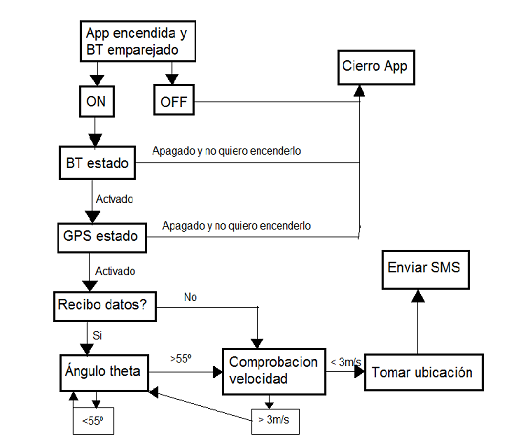
\includegraphics{imagenes/DiagramaEstados.png}
			\caption{Diagrama de Estados}
			\label{contexto:figura}
		\end{figure}
		
		Una vez todo está activado, la aplicación está lista para funcionar, para ello lo primero que hará será leer los datos recibidos por el Handler e interpretarlos. Nuestro algoritmo recibirá los datos ya interpretados, con ellos procederá a calcular el ángulo de inclinación de la motocicleta. Si este ángulo es inferior a 55 grados volvemos a hacer los cálculos con los siguientes datos recibidos. Este proceso se realiza de forma periódica cada 550 milisegundos. En el caso de que éste ángulo sea superior a 55 grados procedemos a comprobar la velocidad de la motocicleta.
		
		Para comprobar la velocidad de la motocicleta se usará el GPS del smartphone, por lo que en este momento se procederá al uso del GPS, para ahorrar batería no lo tendremos encendido durante todo el transcurso del desplazamiento. Si la velocidad medida es mayor a 3 metros por segundo, volvemos al principio del algoritmo y volvemos a calcular el ángulo de inclinación de la motocicleta, en caso de que la velicidad sea menor a 3 metros por segundo procedemos a tomar a la ubicación según las coordenadas de latitud, longitud y precisión.
		
		Estos datos obtenidos por el GPS serán los que enviemos via SMS al número de emergencias, indicándoles la posición actual en latitud, longitud y la precisión con que mide el GPS del smartphone.
		
		En el caso de perder la se\~nal y no recibir datos, el sistema entrará en un proceso de espera temporal, si no se recupera la recepción de datos transcurriendo este tiempo se procederá a calcular la velocidad y seguir con el disgrama de estados según la velocidad. Si durante el transcurso de ese tiempo de espera se pulta el botón OFF la aplicación se cerrará completamente.
	
		
	\section{Aplicación Móvil}
	
		En esta sección procederé a explicar en detalle el desarrollo de la aplicación Android, así como el diagrama de estados del algoritmo implementado y la interfaz eventual para comprobar el funcionamiento correcto de la aplicación.
		
		\subsection{Elección software para el desarrollo de la aplicación}
			
			A la hora de realizar la aplicación que procesará los datos recibidos por el Bluetooth y ejecutará el algoritmo de accidente estudiamos cual es la situación del mercado en lo que respecta al sistema operativo de los dispositivos en uso. 
			
			Según una noticia publicada por xataka en 2014 \cite{AndroidVsiOS} podemos ver los datos proporcionados por la consultora IDC, resultados que se muestran a continuación.
			
			\begin{figure}[h]
				\centering
				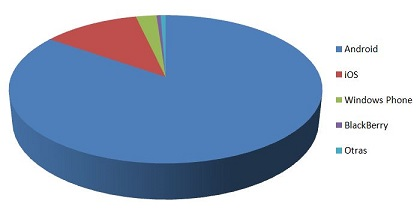
\includegraphics{imagenes/ArduinoVsiOS.jpg}
				\caption{Comparativa Sistema Operativos en uso}
				\label{contexto:figura}
			\end{figure}
			
			En la siguiente tabla mostramos los porcentajes de los dispositivos que usan cada uno de los sistemas operativos disponibles en el mercado.
			
			\begin{table}[H]
				\centering
				\begin{tabular}{p{4cm} p{4cm}}
					\hline
					Sistema Operativo & \% Uso mundial \\
					\hline \hline
					Android & 84.7 \\
					\hline
					iOS & 11.7 \\
					\hline
					Windows Phone & 2.5 \\
					\hline
					BlackBerry & 0.5 \\
					\hline
					Otros & 0.6 \\
					\hline
				\end{tabular}
				\caption{Porcentaje mundial de sistemas operativos en Smartphones}
				\label{tabla:AndroidVsiOS}
			\end{table}
			
			Viendo estos datos se decidió realizar la aplicación para un dispositivo Android.
		
		\subsection{Android}
		
			Para el desarrollo de ésta aplicación hemos descargado el programa Eclipse ADT de Android Developer. Programa que he usado para el desarrollo íntegro de la aplicación MotoSafe. Se debe prestar atención a partir de que versión de Android deseamos implementar la aplicación, escogí la versión Android 4.4 ya que es la que actualmente posee mi smartphone, para una posterior comercialización debo hacer ésta aplicación disponible a partir de la version Android 2.3 ya que la mayoría de los smartphones poseen ésta versión.
			
			En su implementación se ha usado una única clase, que es la clase main, por defecto invocada al ejecutarse el programa y que contiene el bucle que realiza todas las acciones necesarias para que el programa funcione correctamente,  tal y como se muestra en la figura 3.7. 
			
			Aqui debo destacar que en el fichero main no solo contengo la clase main, sino también la clase RecibirComando, que es la encargada de enviar por el Handler toda la información recibida del bluetooth.
		
			\begin{figure}[h]
				\centering
				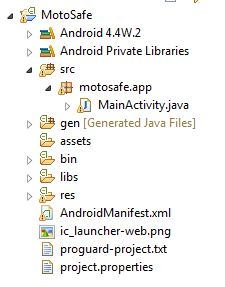
\includegraphics{imagenes/main.JPG}
				\caption{Estructura aplicación Android}
				\label{contexto:figura}
			\end{figure}
			
			En resumen, la clase main será la encargada de gestionar todos los datos recibidos por el Handler, comprobar el estado del GPS, Bluetooth y si ambos dispositivos se encuentran conectados o se pierde la conexión. Además será la clase encargada de ejecutar el algoritmo y en caso necesario registrar la ubicación para posteriormente enviarsela vía SMS a emergencias.
			
			En los próximos apartados se explicará con mas detalle el funcionamiento de la aplicación y se mostrará el diagrama de estados.
				
		
		\subsection{Interfaz Aplicación}
		
			La interfaz eventual de nuestra aplicación es la mostrada en la figura 3.9. En la cual se pueden apreciar dos botones, uno de encendido ON y otro de apagado OFF. Además disponemos de 4 TextView, los cuales usaremos para comprobar el estado actual de la aplicación.
			
			\begin{figure}[h]
				\centering
				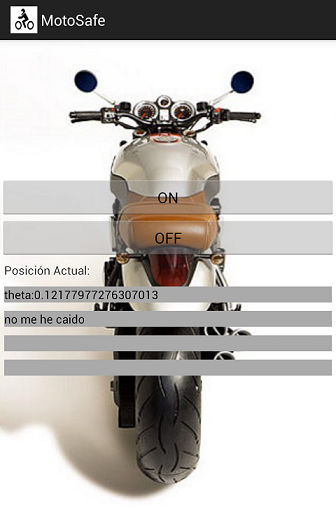
\includegraphics{imagenes/interfaz.png}
				\caption{Interfaz aplicación Android}
				\label{contexto:figura}
			\end{figure}
			
			El primer TextView muestra el ángulo theta de inclinación, siendo su valor entre -90 y 90 grados con respecto a la vertical, dependiendo si estamos inclinados hacia la derecha o hacia la izquierda. El segundo TextView mostrará dos mensajes, uno de ellos ''no me he caido'' y el otro ''es posible que me haya caido'', si el mensaje mostrado es el segundo el tercer TextView mostrará ''comprobando velocidad''. Basándose en el algoritmo implementado, si se ha sufrido un accidente el cuarto y último TextView mostrará el siguiente mensaje ''He sufrido un accidente y mi ubicación es: latitud 'x' longitud 'y' precisión 'z' '' éste será el mensaje que se enviará vía SMS a emergencias, mostrando las coordenadas calculadas con el GPS. En caso de no haber sufrido accidente no se mostrará nada en este último TextView. 
			
			

	\newpage
	$\ $
	